



\documentclass[a4paper,12pt,spanish]{article}

\usepackage[utf8]{inputenc}


\usepackage{blindtext}
%\usepackage{microtype}
\usepackage{amsfonts, amsmath, amsthm, amssymb}
%\usepackage{fancyhdr}
%\usepackage{index}
%\usepackage{multicol}    

%\usepackage{booktabs}

\usepackage[T1]{fontenc}
\usepackage[utf8]{inputenc}
\usepackage{graphicx}
\usepackage[spanish,es-tabla]{babel}
\usepackage{url}
\usepackage{enumitem}

\usepackage[unicode=true, pdfusetitle,
bookmarks=true,bookmarksnumbered=false,bookmarksopen=false,
breaklinks=true,pdfborder={0 0 1},backref=false,colorlinks=false]
{hyperref}

\usepackage{listings}
\usepackage{longtable}


\usepackage{siunitx} %para el sistema internacional
\usepackage[export]{adjustbox}
\usepackage{booktabs} 
\usepackage{subcaption}

\usepackage{float}


\newcommand{\address}[1]{
	\par {\raggedright #1
		\vspace{1.4em}
		\noindent\par}
}

\usepackage[table,xcdraw]{xcolor}


\pagenumbering{gobble}
\include{noNumberPage}
\pagenumbering{arabic}
\setcounter{page}{1}

%tutorial de tablas latex: https://manualdelatex.com/tutoriales/tablas

\usepackage{multirow}

% \usepackage[table,xcdraw]{xcolor}


%Inicio del documento (hasta que se cierre con \end{document}
\begin{document}
	
	
	\title{ Espectroscopía Gamma con detectores de INa(Tl) }
	
	
	%\author{Adrián Rivero Fernández}
	\date{}
	
	\maketitle
	
	
	\section{Objetivos de la práctica}
	
	\vspace{\baselineskip}
	
	1. Medir el fondo radiactivo con el detector cerrado y abierto.\\
	
	2. Calibrar en energías con una fuente radiactiva.\\
	
	3. Determinar la eficiencia del detector, medirla para varias energías y graficar la eficiencia en función de la energía.\\
	
	4. Medir la resolución de diferentes picos y graficar la resolución en función de la energía.\\
	
	5. Estudiar los espectros, determinar teórica y experimentalmente el fotopico, la distribución de Compton y la retrodispersión de cada uespectro.\\
	
	6. Determinar la actividad de la muestra de actividad desconocida.\\
	
	7. Determinar las energías de una muestra desconocida. Determinar su composición.\\
	
	
	\section{Determinación del fondo}
	
	
\begin{figure}[H]
	\centering
	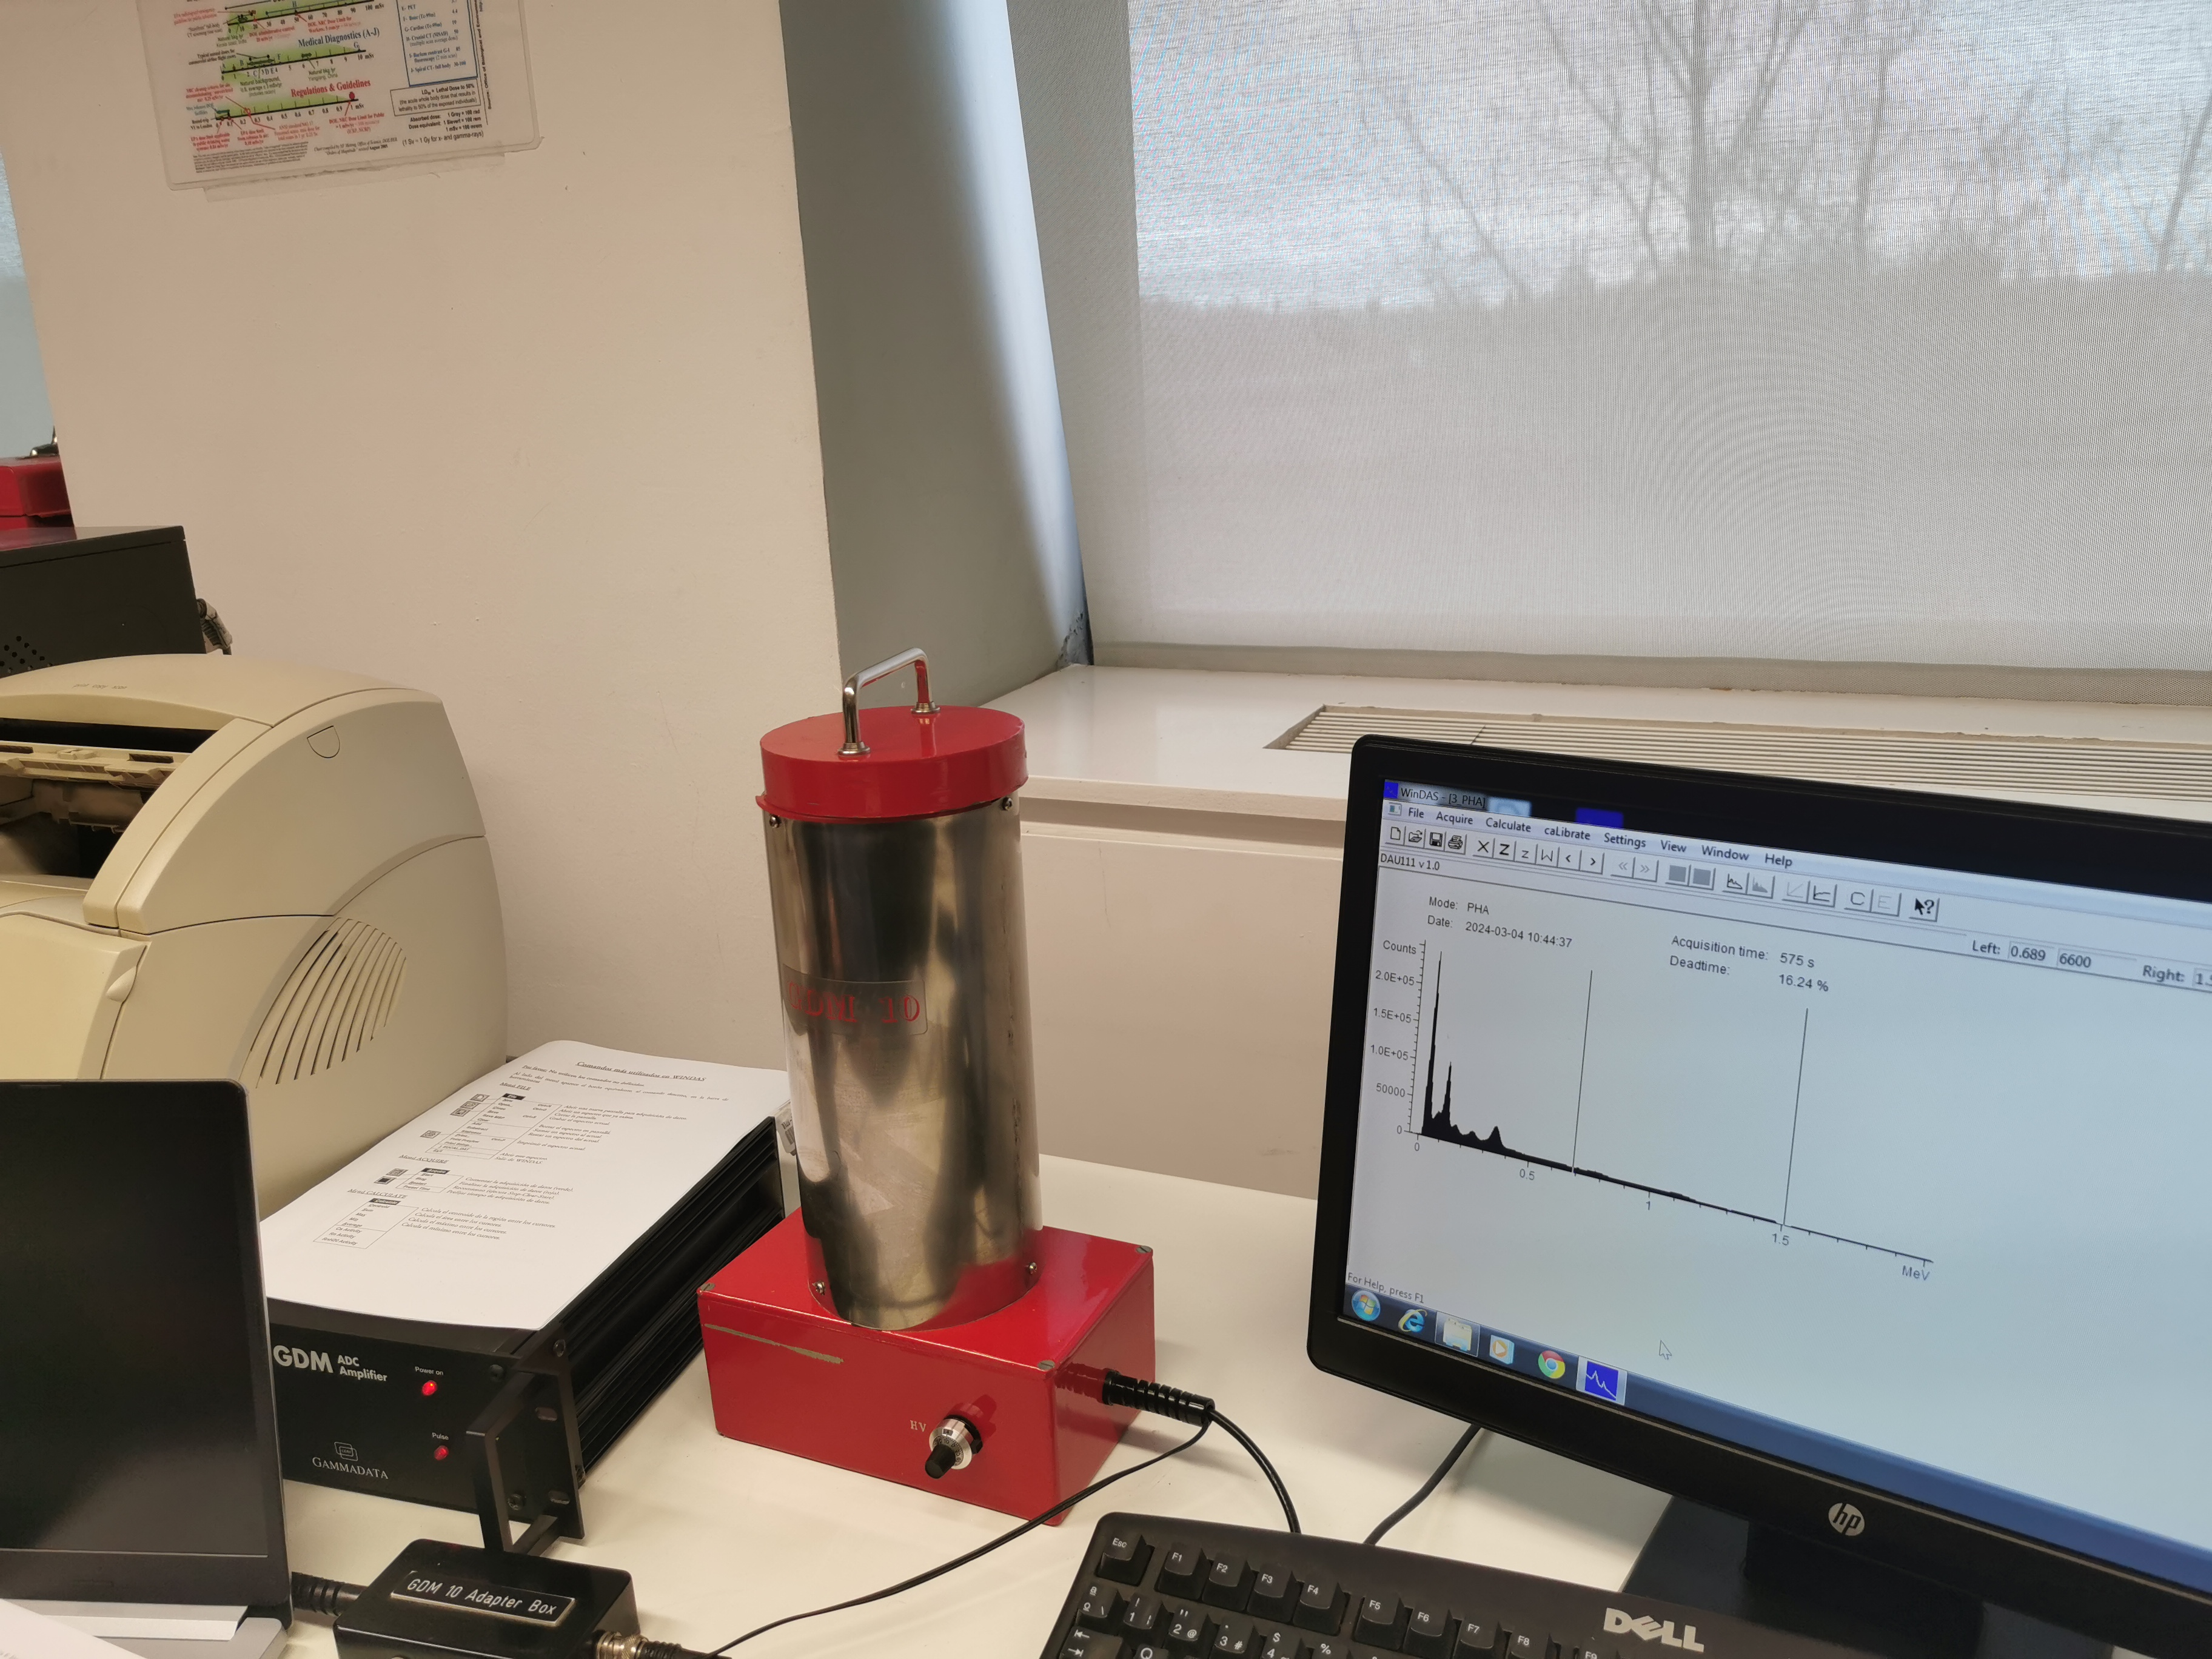
\includegraphics[width=0.7\linewidth]{../IMG_20240304_110653}
	\caption{Detector con su sistema de digitalización.}
	\label{fig:img20240304110653}
\end{figure}

	Iniciamos los aparatos, y tomamos muestras del espectro del fondo con el castillete vacío tapado y destapado.
	
	
\begin{figure}[H]
	\centering
	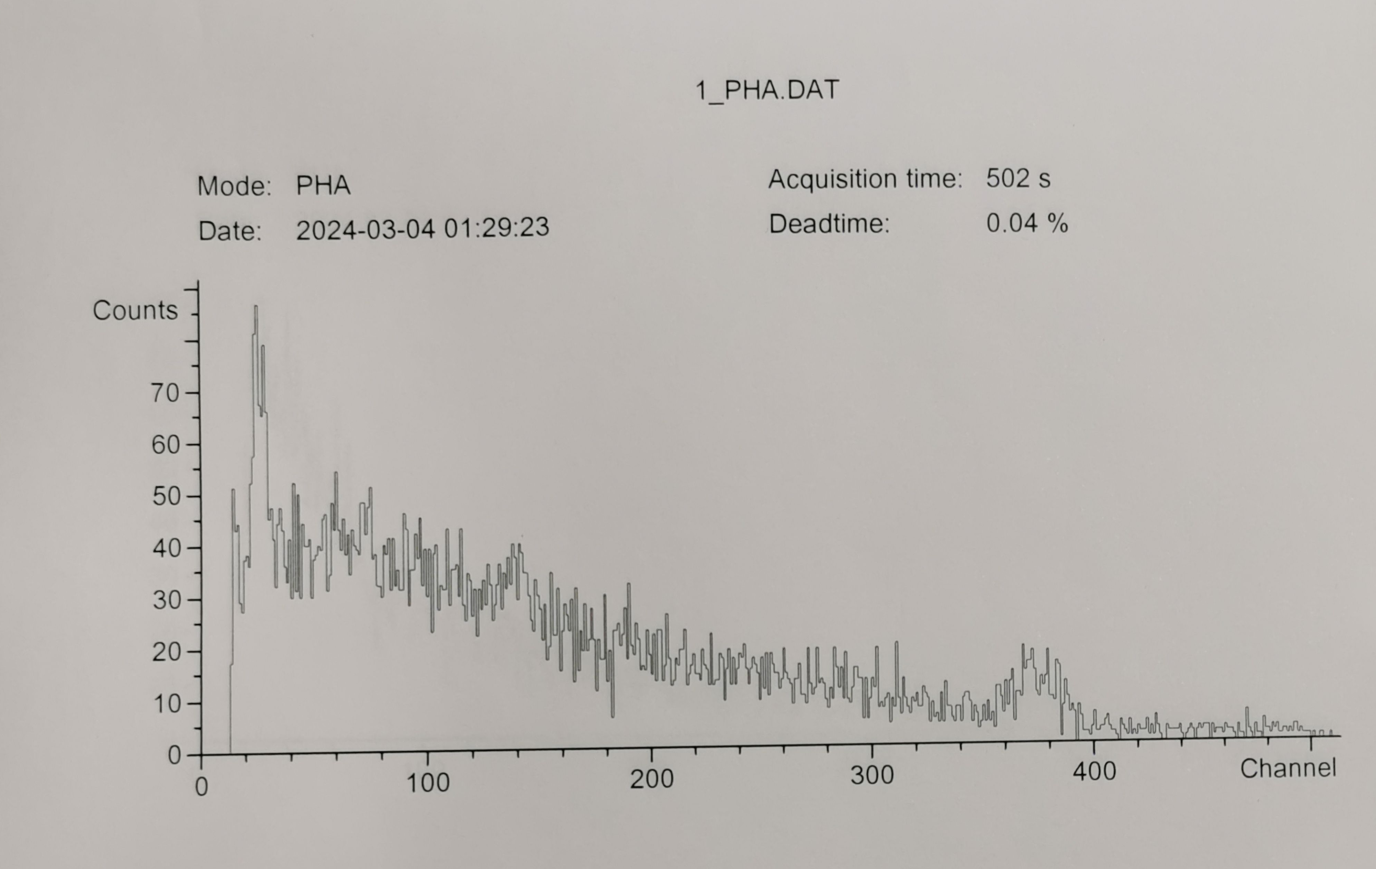
\includegraphics[width=0.7\linewidth]{../graficas_procesadas/PHA_1}
	\caption{Medición de fondo con el castillete tapado}
	\label{fig:pha1}
\end{figure}
	
	
\begin{figure}[H]
	\centering
	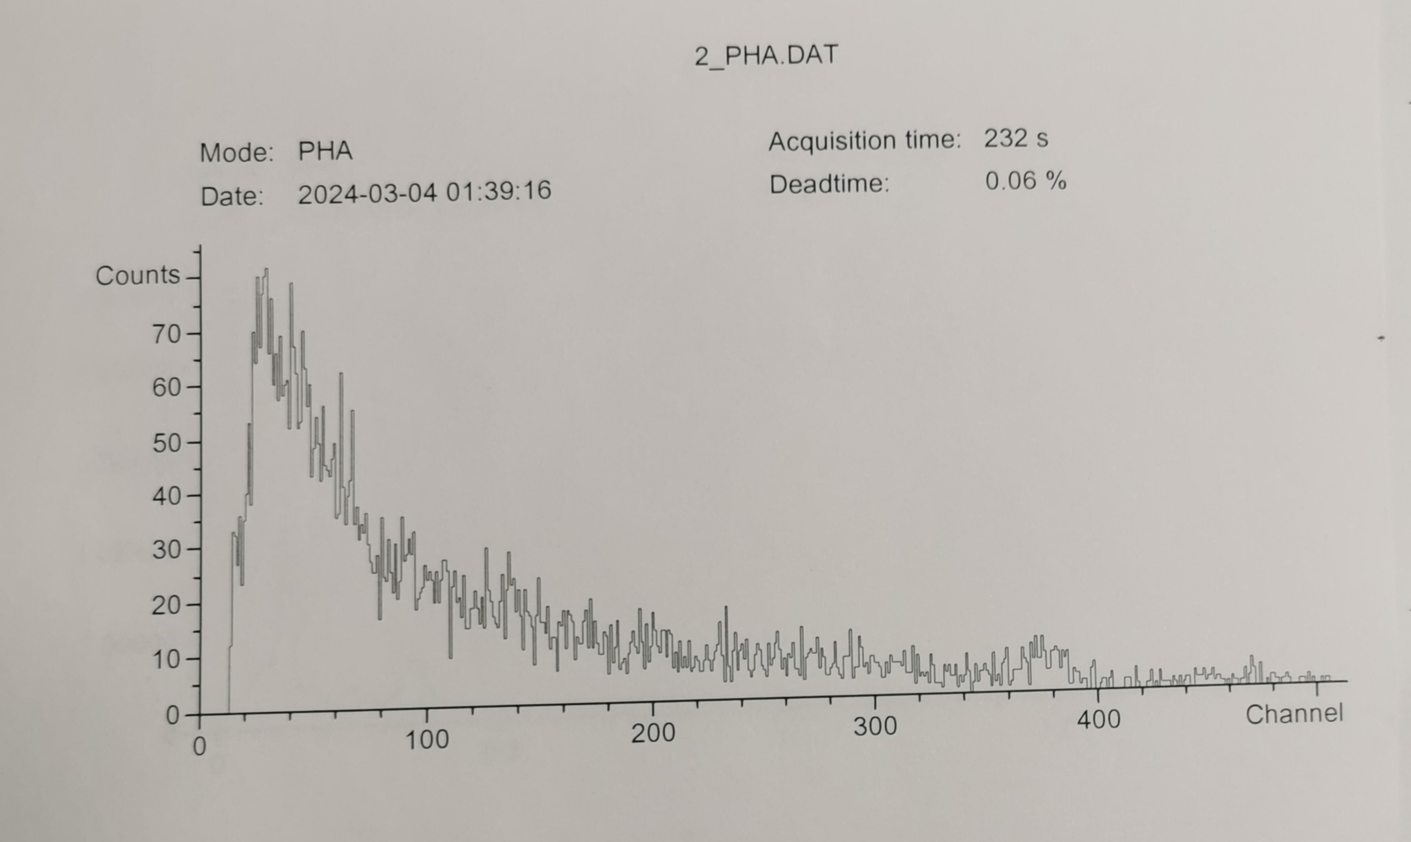
\includegraphics[width=0.7\linewidth]{../graficas_procesadas/PHA_2}
	\caption{Medición de fondo con el castillete destapado}
	\label{fig:pha2}
\end{figure}


[falta comparar y resolver cuestiones]
	
	\section{Calibración de energías}
	
	Tomamos primero el Europio-152, que usaremos para calibrar el detector.
	
	
\begin{figure}[H]
	\centering
	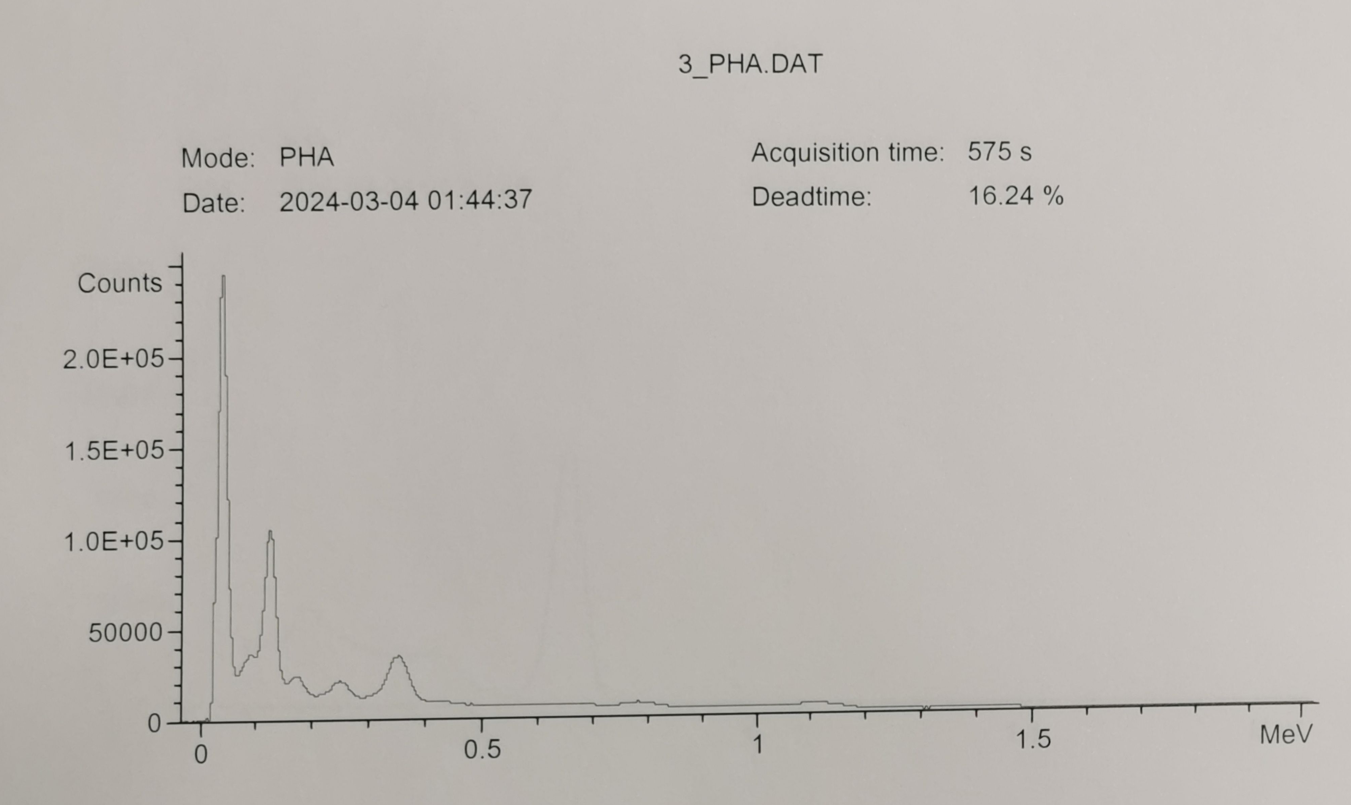
\includegraphics[width=0.7\linewidth]{../graficas_procesadas/PHA_3}
	\caption{Espectro gamma del Europio-152}
	\label{fig:pha3}
\end{figure}
	
	\subsubsection*{1º pico}
	Canal = 
	
	Energía = 
	
	\subsubsection*{2º pico}
	Canal = 
	
	Energía = 
	
	Con estos datos, calibramos y comprobamos el resto de picos del Eu$^{152}$. 
	
	
	
	\section{Eficiencia del detector para las gammas}
	
	Primero calculamos la actividad real de la muestra, teniendo en cuenta que la actividad inicial a 12 de octubre de 2022 era de 1$\mu$Ci, a día 4 de marzo de 2024 (1 año y 5
	meses después):
	\[ A = A_0 \text{e}^{-\frac{\ln2}{T_{1/2}t}}\]
		
	con 
	
	\[A_0 = 1\si{\mu Ci}\]
	\[t = 1,42 \text{años}\]
	\[ T_{1/2} = 13 \text{años}
	\]
	Quedando
	\[ A = 0,927\si{\mu Ci} = 34308,14 \si{Bq}
	\]
	
	Teniendo en cuenta la relación entre la actividad y la eficiencia
	\[ A = \frac{A_f}{\varepsilon(E) C_r} \longrightarrow \varepsilon = \frac{A_f}{A·C_r}
	\]
	siendo $A_f$ el area del fotopico en Bequerelios, $A$ la actividad calibrada, $\varepsilon$ la eficiencia y $C_r$ el coeficiente de ramificación (dado en el guión de prácticas) correspondiente a cada pico.
	
	\begin{table}[H]
		\centering
		\begin{tabular}{|c|c|c|c|c|c|}
			\hline
			$E$ (MeV) & $E$ real (Mev) & $A_f$ (Bq) & Cr    & Eficiencia & Eficiencia (\%) \\ \hline\hline
			0,04      & 0,039          & 2113       & 0,567 & 0,108      & 10,807          \\ \hline
			0,122     & 0,122          & 806        & 0,307 & 0,076      & 7,613           \\ \hline
			0,244     & 0,247          & 112        & 0,079 & 0,041      & 4,111           \\ \hline
			0,344     & 0,351          & 449        & 0,272 & 0,048      & 4,787           \\ \hline
			0,78      & 0,79           & 48,9       & 0,133 & 0,011      & 1,066           \\ \hline
			0,96      & 0,97           & 26,7       & 0,145 & 0,005      & 0,534           \\ \hline
			1,41      & 1,41           & 56,9       & 0,214 & 0,008      & 0,771           \\ \hline
		\end{tabular}
	\caption{Valores de la eficiencia para cada pico de Eu$^{152}$}
	\end{table}
	
	Representando la eficiencia para cada energía de pico:
	
	
\begin{figure}[H]
	\centering
	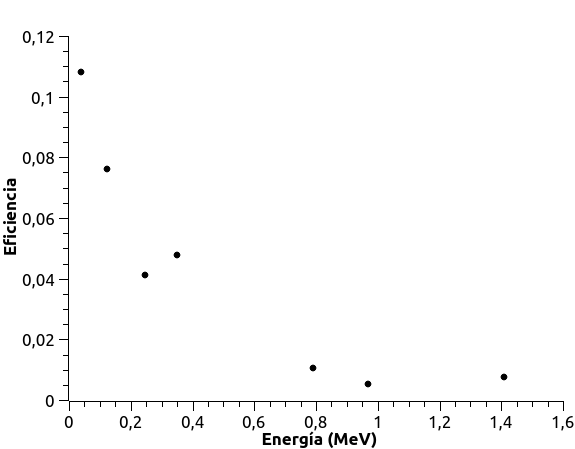
\includegraphics[width=0.7\linewidth]{6_1eficienciaenergia}
	\caption{Eficiencia según energía para el Eu$^{152}$}
	\label{fig:61eficienciaenergia}
\end{figure}
	
	\section{Medida de la resolución}
	
	
	
	\section{Estudio de espectros}
	
	\section{Actividad desconocida}
	
	\section{Muestra desconocida}
	
	
	
	
	
	
	
	
	
	
	
\end{document}






